% !TeX program = pdflatex
\documentclass[10pt,letterpaper]{article}

\usepackage{epigenetics-preprint}

\preprintKicker{bioRxiv preprint}
\preprintCategory{Computational Biology}
\preprintDate{June 2026}
\preprintTitle{EpigeneticsBench: Verifiable Evaluation of AI Agents on Epigenomics Analysis}
\preprintSubtitle{Short-horizon tasks from real epigenomics workflows}
\preprintAuthors{Harihara Muralidharan\preprintSup{1}, Reema Baskar\preprintSup{1}, Soo Hee Lee\preprintSup{1}, Kenny Workman\preprintSup{1}}
\preprintAffiliations{\preprintSup{1}LatchBio, San Francisco, CA, USA}
\preprintCorrespondence{kenny@latch.bio}

\begin{document}

\PreprintHeader

\begin{PreprintAbstract}
We introduce EpigeneticsBench, a verifiable benchmark for short-horizon
epigenomics analysis. Rather than asking agents to produce open-ended
biological interpretations, EpigeneticsBench evaluates whether they can
execute focused analysis decisions from realistic workflow states and return
deterministically gradable answers. The updated benchmark includes 106
evaluations across CUT\&Tag/CUT\&RUN, ATAC-seq, ChIP-seq, and DNA methylation
workflows. Across 5,088 parsed trajectories from 16 model-harness pairs, no
system solves a majority of attempts: GPT-5.5 / Pi leads at 151/318 attempts
(47.5\%), followed by GPT-5.5 / OpenAI Codex at 135/318 attempts (42.5\%) and
GPT-5.4 / Pi at 134/318 attempts (42.1\%). Difficulty is structured by assay
source and workflow convention more than by nominal horizon label, and
component-level scoring reveals frequent partial recovery despite endpoint
failure. These results suggest that current agents can often locate and
manipulate the right biological evidence, but still fail at brittle local
decisions involving metric definitions, comparator scope, normalization state,
and answer-surface constraints.
\end{PreprintAbstract}

\vfill
\clearpage

\section*{Topline Benchmark Performance}

{\fontsize{9.1}{12.8}\selectfont
We ran the benchmark across 16 model-harness pairs. Pi denotes the Pi terminal
coding harness. Passing requires exact recovery of the graded structured
answer for an evaluation attempt. The updated manifest contains 5,088 valid
result JSONs in a balanced three-replicate design: 106 evaluations for each of
16 model-harness pairs.
\par}

\begin{center}
  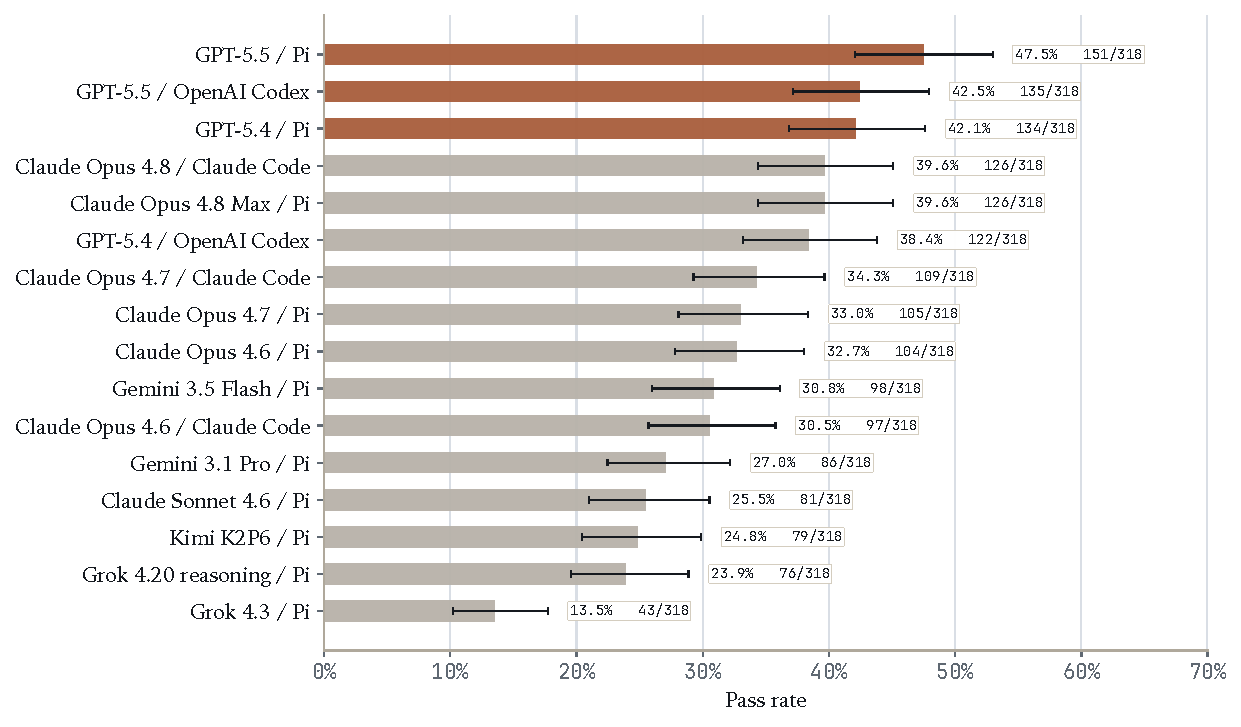
\includegraphics[width=0.94\textwidth]{figures/topline/figA_pass_rate_by_model.pdf}

  \vspace{0.18in}

  \begin{minipage}[t]{0.485\textwidth}
    \centering
    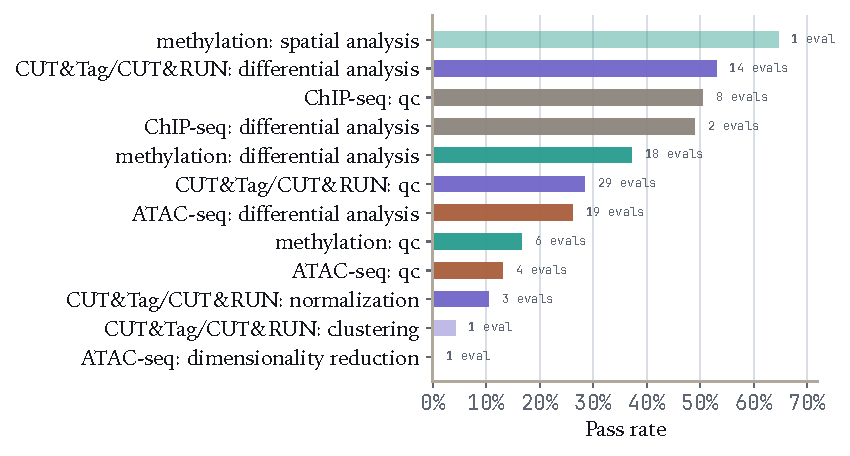
\includegraphics[width=\linewidth]{figures/topline/figB_pass_rate_by_kit_task.pdf}
  \end{minipage}
  \hfill
  \begin{minipage}[t]{0.485\textwidth}
    \centering
    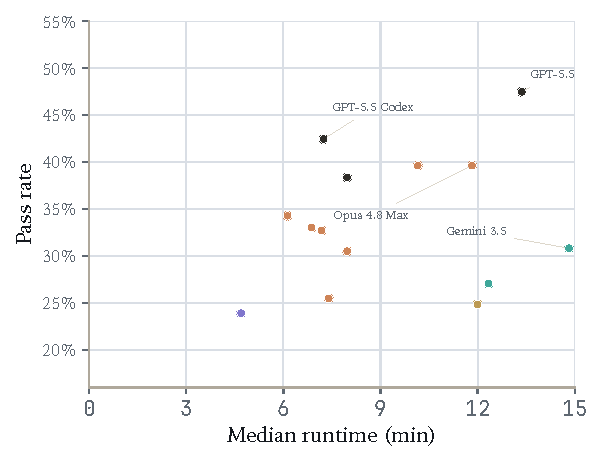
\includegraphics[width=\linewidth]{figures/topline/figC_pass_rate_vs_runtime.pdf}
  \end{minipage}

  \captionof{figure}{\textbf{Topline benchmark performance.}
  Top: run-level pass rate by model-harness pair across all parsed attempts.
  Bottom left: pass rate by assay and task family. Bottom right: pass rate
  against median runtime. Wilson confidence intervals and evaluation-level
  replicate statistics are reported in Table~\ref{tab:model-results}.}
  \label{fig:topline-performance}
\end{center}

\StartBody

\section{Introduction}

Epigenomics connects regulatory sequence, chromatin accessibility, histone
modification, DNA methylation, and genome organization to cell state and gene
regulation. Modern assays can measure these layers at population,
single-cell, and spatial resolution, but the resulting analyses are brittle:
small choices in genome build, peak filtering, motif background selection,
sample aggregation, or denominator definition can change a biological
conclusion \cite{encode2012,roadmap2015,buenrostro2013,kayaokur2019}.

AI agents can now inspect files, write analysis code, run command-line tools,
and return structured biological summaries. Benchmarks have therefore moved
from question answering toward executable scientific tasks. SpatialBench tests
localized spatial biology analysis, scBench tests single-cell workflows, and
SpatialBench-Long tests recovery of complex scientific conclusions from raw
or near-raw spatial data
\cite{workman2025spatialbench,workman2026scbench,workman2026spatialbenchlong}.

Epigenomics needs a complementary short-horizon benchmark. Many consequential
failures occur in compact analysis decisions rather than in full-project
autonomy: deciding which count layer to use, whether a statistic should be
computed per peak, per gene, or per sample, which contrast is biologically
appropriate, or how a CpG, motif, or chromatin-state summary should be
normalized.

This benchmark evaluates those local empirical decisions. Each task snapshots
a realistic analysis state immediately before a target result. The agent must
interact with the provided data and return a structured answer that can be
graded deterministically. The benchmark is therefore not a test of broad
regulatory-biology plausibility. It asks whether an agent can produce the
specific verifiable result supported by the data, assay context, and requested
answer surface.

\EndBody

\section{Benchmark Design}

{\fontsize{9.1}{12.8}\selectfont
The benchmark contains 106 evaluations derived from practical epigenomics
analysis workflows. Tasks are short-horizon: they isolate one focused
analysis decision while preserving enough real data context that a model must
inspect files, choose the relevant representation, and compute or verify the
requested result. The benchmark follows the SpatialBench convention of
withholding the full task set to reduce contamination while reporting
aggregate model results and releasing representative examples.
\par}

{\fontsize{9.1}{12.8}\selectfont
\begin{center}
\begin{tikzpicture}
  \node[
    fill=figurecream,
    draw=figureline,
    line width=0.45pt,
    rounded corners=8pt,
    inner xsep=0.20in,
    inner ysep=0.14in,
    text width=0.91\textwidth,
    align=left
  ] {%
    \begin{minipage}{0.91\textwidth}
      {\fontsize{8.5}{10}\selectfont\bfseries\color{paperaccent}Benchmark Construction Workflow}\par
      \vspace{0.08in}
      \centering
      \resizebox{0.84\textwidth}{!}{%
      \begin{tikzpicture}[x=1in,y=1in,>=stealth]
        \node[draw=figureline,fill=white,rounded corners=5pt,inner sep=5pt,
          text width=1.35in,align=center] (a) at (0,0)
          {\fontsize{7.2}{8.5}\selectfont\bfseries Snapshot workflow state\\
          \normalfont real assay outputs and metadata};
        \node[draw=figureline,fill=white,rounded corners=5pt,inner sep=5pt,
          text width=1.35in,align=center] (b) at (1.85,0)
          {\fontsize{7.2}{8.5}\selectfont\bfseries Define target decision\\
          \normalfont one empirical result};
        \node[draw=figureline,fill=white,rounded corners=5pt,inner sep=5pt,
          text width=1.35in,align=center] (c) at (3.70,0)
          {\fontsize{7.2}{8.5}\selectfont\bfseries Constrain answer surface\\
          \normalfont endpoint grader};
        \node[draw=figureline,fill=white,rounded corners=5pt,inner sep=5pt,
          text width=1.35in,align=center] (d) at (5.55,0)
          {\fontsize{7.2}{8.5}\selectfont\bfseries Inspect failures\\
          \normalfont metric and comparator traps};
        \draw[->,line width=0.45pt,color=paperaccent] (a.east) -- (b.west);
        \draw[->,line width=0.45pt,color=paperaccent] (b.east) -- (c.west);
        \draw[->,line width=0.45pt,color=paperaccent] (c.east) -- (d.west);
      \end{tikzpicture}
      }
      \captionof{figure}{\textbf{Benchmark construction workflow.}
      Short-horizon epigenomics evaluations are built by selecting real
      analysis snapshots, defining a single verifiable target decision,
      constraining the final answer schema, and using trajectory inspection to
      identify shortcut-prone or under-specified tasks.}
      \label{fig:construction-workflow}
    \end{minipage}
  };
\end{tikzpicture}
\end{center}
}

{\fontsize{9.1}{12.8}\selectfont
\begin{multicols}{2}

The benchmark is organized around analysis states rather than independent
datasets. A single source study or workflow can contribute multiple
evaluations that vary the target statistic, comparator, or biological claim.
This mirrors how working epigenomics analyses proceed: a scientist repeatedly
queries the same assay context to answer adjacent but distinct questions.

Tasks are designed to specify \emph{what} should be recovered rather than
\emph{how} it should be recovered. Some procedural evaluations name an
operation directly, but most scientific evaluations leave room for the agent
to choose reasonable commands, scripts, and summary logic. This prevents the
prompt from becoming a hidden solution path while keeping the answer surface
verifiable.

The updated inventory contains 97 scientific evaluations and 9 procedural
evaluations. Most graders are numeric tolerance checks (97/106 evaluations),
with 9 all-of graders for compound structured answers. Component field scores
are retained for diagnostics, but run-level pass/fail is the benchmark score.
This distinction matters because some grader score fields are not normalized
across all evaluations, whereas pass/fail has a consistent interpretation.

Manual trajectory inspection is used in the same spirit as SpatialBench and
SpatialBench-Long: not to replace deterministic endpoint grading, but to make
failure modes legible. The current metadata marks recurring traps such as
wrong comparator or baseline, feature-namespace mismatch, wrong data layer,
metric-definition mismatch, and prior-driven biological overinterpretation.

\end{multicols}
}

\clearpage

\section[Motivating Example: One Local Decision Can Change the Answer]{Motivating Example: One Local Decision Can Change\\ the Answer}

{\fontsize{9.1}{12.8}\selectfont
\begin{center}
\begin{tikzpicture}
  \node[
    fill=figurecream,
    draw=figureline,
    line width=0.45pt,
    rounded corners=8pt,
    inner xsep=0.20in,
    inner ysep=0.14in,
    text width=0.88\textwidth,
    align=left
  ] {%
    \begin{minipage}{0.88\textwidth}
      {\fontsize{8.5}{10}\selectfont\bfseries\color{paperaccent}Short-Horizon Epigenomics Chokepoints}\par
      \vspace{0.08in}
      \centering
      \resizebox{0.82\textwidth}{!}{%
      \begin{tikzpicture}[x=1in,y=1in,>=stealth]
        \node[draw=figureline,fill=white,rounded corners=5pt,inner sep=5pt,
          text width=1.25in,align=center] (a) at (0,0)
          {\fontsize{7.2}{8.5}\selectfont\bfseries Assay layer\\
          \normalfont peak, CpG, motif, or gene};
        \node[draw=figureline,fill=white,rounded corners=5pt,inner sep=5pt,
          text width=1.25in,align=center] (b) at (1.72,0)
          {\fontsize{7.2}{8.5}\selectfont\bfseries Comparator\\
          \normalfont condition, subtype, or sample};
        \node[draw=figureline,fill=white,rounded corners=5pt,inner sep=5pt,
          text width=1.25in,align=center] (c) at (3.44,0)
          {\fontsize{7.2}{8.5}\selectfont\bfseries Unit\\
          \normalfont field, feature, or replicate};
        \node[draw=figureline,fill=white,rounded corners=5pt,inner sep=5pt,
          text width=1.25in,align=center] (d) at (5.16,0)
          {\fontsize{7.2}{8.5}\selectfont\bfseries Schema\\
          \normalfont exact structured answer};
        \draw[->,line width=0.45pt,color=paperaccent] (a.east) -- (b.west);
        \draw[->,line width=0.45pt,color=paperaccent] (b.east) -- (c.west);
        \draw[->,line width=0.45pt,color=paperaccent] (c.east) -- (d.west);
      \end{tikzpicture}
      }
      \captionof{figure}{\textbf{Short-horizon epigenomics chokepoints.}
      A representative evaluation snapshots an analysis immediately before a
      local decision. Agents must identify the relevant assay layer, choose the
      requested comparison, compute the target statistic over the correct unit
      of analysis, and return a constrained answer that can be graded
      deterministically.}
      \label{fig:epigenomics-chokepoints}
    \end{minipage}
  };
\end{tikzpicture}
\end{center}

\begin{multicols}{2}

The short-horizon setting is easiest to see through a single evaluation. One
representative ATAC-seq task begins after peak-level outputs and sample
metadata have already been staged. The agent is not asked to reconstruct an
entire study; it must choose the correct representation, comparator,
denominator, and final answer schema for one constrained empirical result.

This kind of task is small enough to be verifiable but still scientifically
fragile. A trajectory can inspect the right files and compute a plausible
statistic, yet fail by using the wrong feature namespace, aggregating over the
wrong biological unit, or substituting a nearby biological contrast for the
requested one. Conversely, a passing answer requires more than memorized
regulatory biology: it requires matching the requested output to the data
layer and comparison actually supplied in the task.

This example illustrates why deterministic endpoint grading and diagnostic
metadata are both useful. The benchmark score remains binary, because the
target answer is a constrained scientific artifact. The failure analysis asks
which local decision broke when the endpoint answer was wrong.

\end{multicols}
}

\clearpage

\section{Evaluation Inventory}

{\fontsize{9.1}{12.8}\selectfont
The benchmark covers four assay labels and six task families. CUT\&Tag/CUT\&RUN
tasks are drawn from zebrafish chromatin workflow snapshots and emphasize
quality control, differential chromatin or expression summaries,
normalization, and one clustering task. ATAC-seq tasks cover B-ALL and
cold-response analyses, while ChIP-seq tasks focus on quality-control and
differential histone-mark summaries. Methylation tasks are dominated by
GSE149608 and GSE149609 outputs, including CpG reports, coverage tables,
noncanonical methylation checks, and differential methylation summaries.
\par}

\begin{center}
\fontsize{7.2}{8.7}\selectfont
\setlength{\tabcolsep}{3.2pt}
\begin{tabular}{@{}>{\raggedright\arraybackslash}p{0.16\linewidth}
                >{\centering\arraybackslash}p{0.055\linewidth}
                >{\raggedright\arraybackslash}p{0.25\linewidth}
                >{\raggedright\arraybackslash}p{0.33\linewidth}
                >{\raggedright\arraybackslash}p{0.13\linewidth}@{}}
\toprule
Assay label & Evals & Sources & Task families & Horizon \\
\midrule
CUT\&Tag/CUT\&RUN &
47 &
Zebrafish chromatin workflow snapshots &
QC (29), differential analysis (14), normalization (3), clustering (1) &
Small (47) \\
\addlinespace
ATAC-seq &
24 &
B-ALL ATAC, cold-response ATAC &
Differential analysis (19), QC (4), dimensionality reduction (1) &
Small (24) \\
\addlinespace
ChIP-seq &
10 &
ChIP-seq workflow snapshots &
QC (8), differential analysis (2) &
Small (9), long (1) \\
\addlinespace
DNA methylation &
25 &
GSE149608, GSE149609 &
Differential analysis (18), QC (6), spatial analysis (1) &
Long (25) \\
\bottomrule
\end{tabular}
\captionof{table}{\textbf{Evaluation inventory.}
The short-horizon epigenomics benchmark groups evaluations by assay label while
varying the source workflow, task family, and expected answer surface within
each group.}
\label{tab:evaluation-inventory}
\end{center}

{\fontsize{8.3}{11.4}\selectfont
Across all 106 evaluations, 47 are QC tasks, 53 are differential-analysis
tasks, 3 are normalization tasks, and one each tests dimensionality reduction,
clustering, and spatial analysis. The updated result manifest contains 5,088
valid trajectories from 16 model-harness pairs, with exactly 318 attempts per
model-harness pair.
\par}

\StartBody

\section{Results}

\subsection{Endpoint grading identifies a leading tier rather than a fully ordered leaderboard}

Across 16 model-harness pairs and 5,088 valid trajectories, deterministic
final-answer grading produced 1,672 passes (32.9\%). Success was concentrated
but not cleanly separated across the leading systems. GPT-5.5 / Pi achieved
the highest pass rate, passing 151/318 attempts (47.5\%; Wilson 95\%
confidence interval (CI), 42.1--53.0). GPT-5.5 / OpenAI Codex followed at
135/318 attempts (42.5\%; 37.1--47.9), while GPT-5.4 / Pi reached 134/318
attempts (42.1\%; 36.8--47.6). Claude Opus 4.8 Max / Pi and Claude Opus 4.8 /
Claude Code both passed 126/318 attempts (39.6\%).

The updated manifest is balanced: each model-harness pair contributes three
rounds for each of 106 evaluations. The middle panel of
Figure~\ref{fig:main-results-summary} therefore matches the full parsed
set rather than a smaller sensitivity subset. The practical interpretation is
unchanged from the earlier draft but sharper: GPT-5.5 / Pi is the descriptive
leader, while the nearby systems form a leading tier whose Wilson intervals
overlap.

\EndBody

\begin{center}
  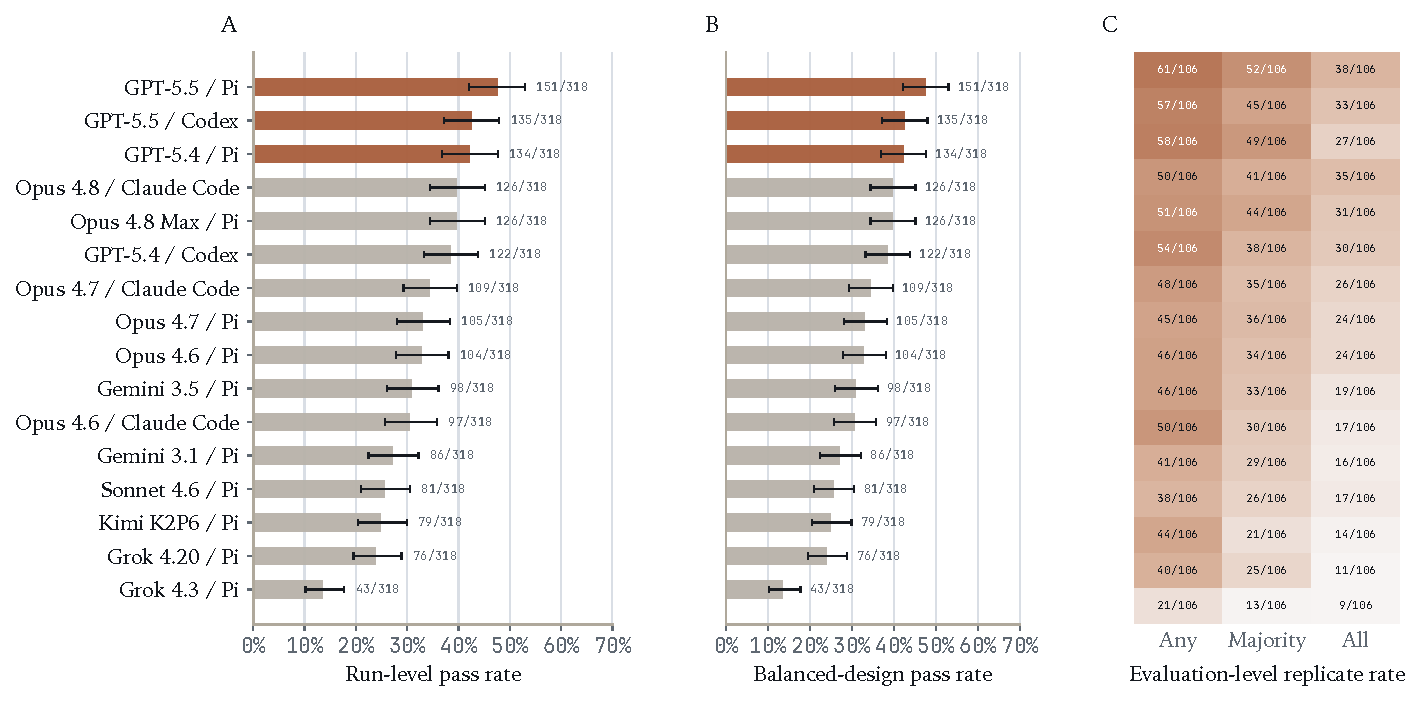
\includegraphics[width=0.94\textwidth]{figures/results/main_results_summary.pdf}

  \captionof{figure}{\textbf{Endpoint success across balanced model-harness
  coverage.} Left: pass rate by model-harness pair across all 5,088 parsed
  attempts. Middle: the same balanced 318-attempt design displayed as a
  shared-instance check. Right: evaluation-level replicate statistics,
  reporting the fraction of attempted evaluations with at least one passing
  attempt, a majority of passing attempts, or all available attempts passing.
  Wilson intervals summarize run-level uncertainty and do not account for
  evaluation-level clustering.}
  \label{fig:main-results-summary}
\end{center}

\vspace{0.08in}

\begin{center}
{\fontsize{4.85}{6.0}\selectfont
\begin{tabular}{@{}>{\raggedright\arraybackslash}p{0.31\linewidth}rrrrrrrr@{}}
\toprule
Model / harness & Pass runs & Pass \% & Wilson 95\% CI & Any & Majority & All & Cost & Median min \\
\midrule
GPT-5.5 / Pi & 151/318 & 47.5 & 42.1--53.0 & 61/106 & 52/106 & 38/106 & \$1.284 & 13.4 \\
GPT-5.5 / OpenAI Codex & 135/318 & 42.5 & 37.1--47.9 & 57/106 & 45/106 & 33/106 & -- & 7.2 \\
GPT-5.4 / Pi & 134/318 & 42.1 & 36.8--47.6 & 58/106 & 49/106 & 27/106 & \$0.924 & 15.3 \\
Claude Opus 4.8 Max / Pi & 126/318 & 39.6 & 34.4--45.1 & 50/106 & 41/106 & 35/106 & -- & 11.8 \\
Claude Opus 4.8 / Claude Code & 126/318 & 39.6 & 34.4--45.1 & 51/106 & 44/106 & 31/106 & -- & 10.2 \\
GPT-5.4 / OpenAI Codex & 122/318 & 38.4 & 33.2--43.8 & 54/106 & 38/106 & 30/106 & -- & 8.0 \\
Claude Opus 4.7 / Claude Code & 109/318 & 34.3 & 29.3--39.7 & 48/106 & 35/106 & 26/106 & -- & 6.1 \\
Claude Opus 4.7 / Pi & 105/318 & 33.0 & 28.1--38.4 & 45/106 & 36/106 & 24/106 & -- & 6.9 \\
Claude Opus 4.6 / Pi & 104/318 & 32.7 & 27.8--38.0 & 46/106 & 34/106 & 24/106 & \$0.620 & 7.2 \\
Gemini 3.5 Flash / Pi & 98/318 & 30.8 & 26.0--36.1 & 46/106 & 33/106 & 19/106 & \$1.587 & 14.8 \\
Claude Opus 4.6 / Claude Code & 97/318 & 30.5 & 25.7--35.8 & 50/106 & 30/106 & 17/106 & -- & 8.0 \\
Gemini 3.1 Pro / Pi & 86/318 & 27.0 & 22.5--32.2 & 41/106 & 29/106 & 16/106 & \$0.768 & 12.3 \\
Claude Sonnet 4.6 / Pi & 81/318 & 25.5 & 21.0--30.5 & 38/106 & 26/106 & 17/106 & \$0.609 & 7.4 \\
Kimi K2P6 / Pi & 79/318 & 24.8 & 20.4--29.9 & 44/106 & 21/106 & 14/106 & \$0.460 & 12.0 \\
Grok 4.20 reasoning / Pi & 76/318 & 23.9 & 19.5--28.9 & 40/106 & 25/106 & 11/106 & \$0.280 & 4.7 \\
Grok 4.3 / Pi & 43/318 & 13.5 & 10.2--17.7 & 21/106 & 13/106 & 9/106 & \$0.033 & 0.7 \\
\bottomrule
\end{tabular}
}

\captionof{table}{\textbf{Deterministic final-answer performance.}
Run-level pass rates are computed over the balanced updated manifest. Any,
Majority, and All report evaluation-level replicate statistics over 106
evaluations for each model-harness pair. Cost is shown only
when it is present for all attempts from that model-harness pair; dashes
indicate incomplete or unavailable cost metadata. Median minutes summarizes
the recorded result duration.}
\label{tab:model-results}
\end{center}

\clearpage

\StartBody

\subsection{Assay source stratifies difficulty more clearly than horizon labels}

Performance varied more by assay source and workflow provenance than by the
coarse horizon label. ChIP-seq tasks passed at 241/480 attempts (50.2\%),
followed by CUT\&Tag/CUT\&RUN at 768/2,256 (34.0\%), methylation at 400/1,200
(33.3\%), and ATAC-seq at 263/1,152 (22.8\%). Source-level summaries exposed a
sharper split within these assay labels: GSE149608 methylation tasks passed at
388/1,152 attempts (33.7\%), whereas the single GSE149609 task passed at
12/48 (25.0\%). Cold-response ATAC tasks passed at 147/576 (25.5\%), while
B-ALL ATAC-prefix tasks passed at 116/576 (20.1\%).

Task family alone was less informative. Differential-analysis tasks passed at
962/2,544 attempts (37.8\%), while QC tasks passed at 662/2,256 (29.3\%).
However, the same nominal task family behaved differently across assay
contexts: CUT\&Tag/CUT\&RUN differential-analysis tasks passed at 356/672
attempts (53.0\%), while ATAC-seq differential-analysis tasks passed at
238/912 (26.1\%). Agents are therefore not simply failing broad task types;
they are sensitive to the representation, comparator, and denominator
conventions of particular epigenomics workflows.

The horizon label should be interpreted cautiously. Long-horizon evaluations
passed at 429/1,248 attempts (34.4\%) versus 1,243/3,840 (32.4\%) for
small-horizon evaluations, but the long group is almost entirely methylation:
all 25 methylation evaluations are long horizon, whereas all CUT\&Tag/CUT\&RUN
and ATAC-seq evaluations are small horizon and only one ChIP-seq evaluation is
long horizon (Figure~\ref{fig:source-horizon-summary}). The small
long-horizon advantage is consequently a source-composition effect rather than
evidence that longer tasks are intrinsically easier.

\EndBody

\begin{center}
  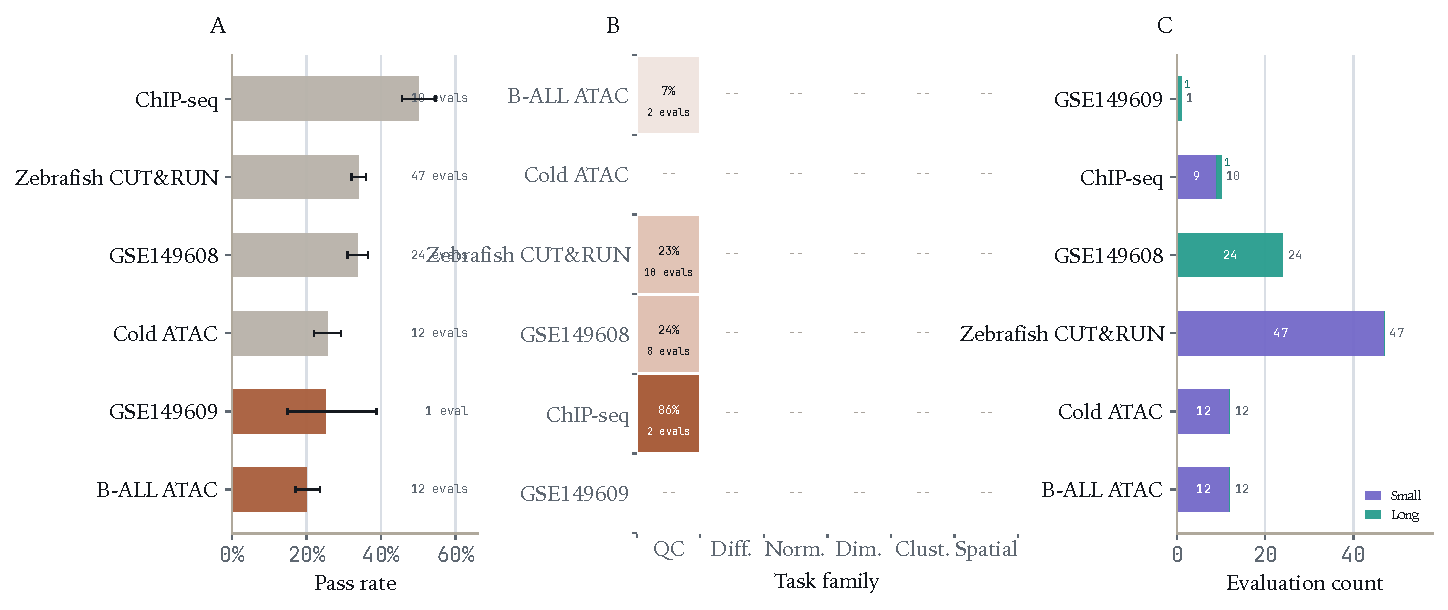
\includegraphics[width=0.88\textwidth]{figures/results/source_and_horizon_summary.pdf}

  \captionof{figure}{\textbf{Performance varies by source workflow and is
  confounded with horizon.} Left: pass rate by source prefix with run-level
  Wilson intervals. Middle: source-by-task pass-rate heatmap; cell text reports
  pass rate and evaluation count. Right: horizon composition by source prefix.
  Long-horizon evaluations are mostly methylation/GSE149608, so the higher
  long-horizon pass rate should not be interpreted as evidence that longer
  tasks are intrinsically easier.}
  \label{fig:source-horizon-summary}
\end{center}

\StartBody

\subsection{Replicate statistics distinguish occasional recovery from stable recovery}

Run-level pass rates are useful for ranking systems, but evaluation-level
replicate statistics better capture reliability. GPT-5.5 / Pi passed at least
one attempt on 61/106 evaluations, passed a majority of attempts on 52/106,
and passed all three attempts on 38/106. GPT-5.5 / OpenAI Codex showed a
similar drop from 57/106 any-pass evaluations to 45/106 majority-pass and
33/106 all-pass evaluations. In contrast, Grok 4.3 / Pi passed at least one
attempt on 21/106 evaluations and a majority on 13/106.

This gap matters because short-horizon tasks are not purely deterministic from
the agent's perspective. A model can know the relevant assay logic but choose
the wrong field name, denominator, or comparator in one replicate. Conversely,
a single passing replicate does not imply stable operational competence. We
therefore treat any-pass rates as evidence of reachable capability and
majority/all-pass rates as stronger evidence of repeatable recovery.

\subsection{Hard evaluations often reflect component conjunction failures}

Evaluation difficulty was highly skewed. Across 106 evaluations, 21 had no
passing attempts and 18 more had pass rates below 10\%, whereas no evaluation
was passed by every available attempt and only three exceeded 90\% pass rate.
The hardest evaluations were not uniformly cases of no analysis progress: 17
of 21 zero-pass evaluations had nonzero mean grader score, and 9 of 21 had
field-level pass rates of at least 50\%.

Field scores show that many failures occur at the final conjunction of
components. Across all 5,088 runs, endpoint pass/fail was exactly equivalent
to all component fields passing. The weighted field-level pass rate was
69.6\%, while endpoint pass rate was 32.9\%. This gap was largest for
ATAC-seq dimensionality reduction, CUT\&Tag/CUT\&RUN normalization, ATAC-seq
QC, CUT\&Tag/CUT\&RUN clustering, CUT\&Tag/CUT\&RUN QC, and ATAC-seq
differential-analysis tasks. These results indicate that many agents recover
substantial local structure but miss one required field, comparator,
denominator, or answer-surface constraint.

\EndBody

\begin{center}
  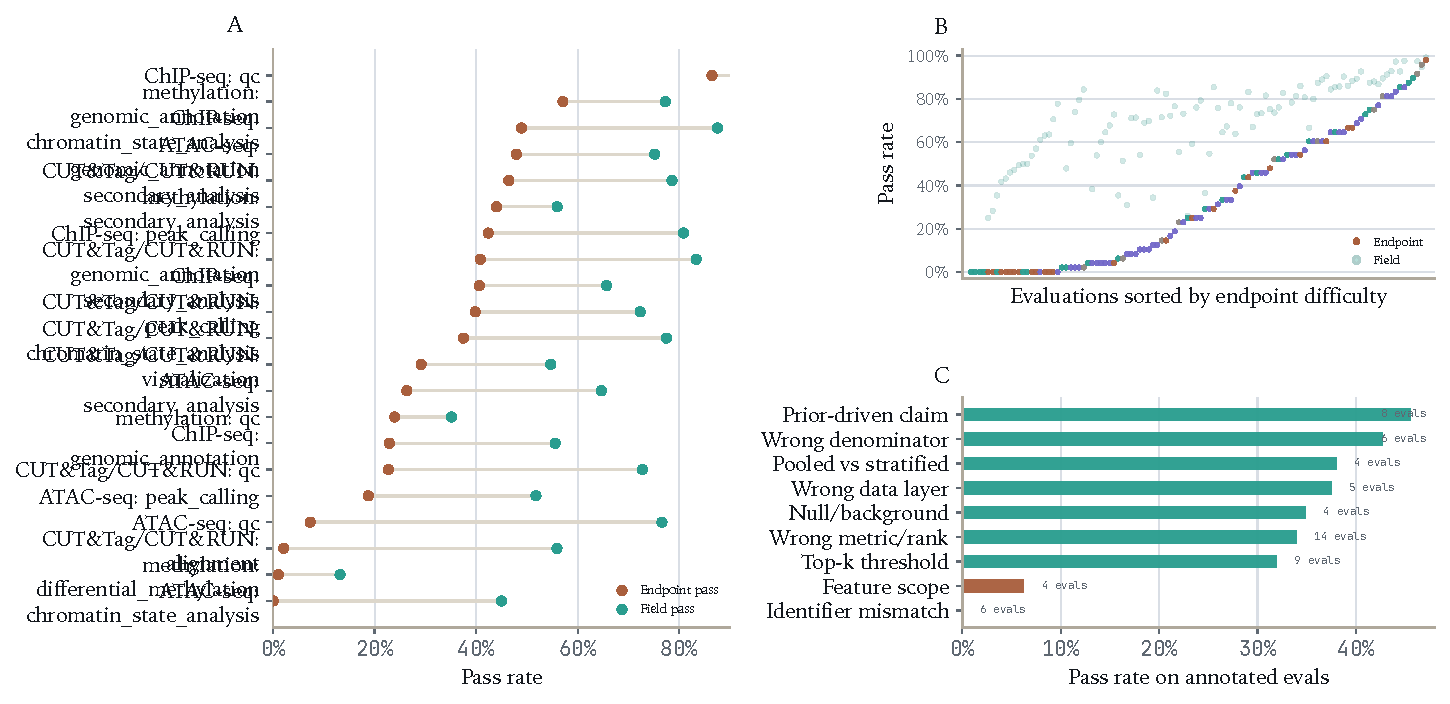
\includegraphics[width=0.92\textwidth]{figures/results/partial_credit_failure_diagnostics.pdf}

  \captionof{figure}{\textbf{Endpoint failures often contain substantial
  partial progress.} Left: endpoint pass rate and field-level pass rate by assay
  and task family. Top right: evaluation-level difficulty spectrum, with
  endpoint pass rate and field-level pass rate shown for each evaluation.
  Bottom right: annotated failure-mode severity; dot size indicates the number
  of uniquely annotated evaluations. Field scores and failure annotations are
  diagnostics, not replacement benchmark scores.}
  \label{fig:partial-credit-failure-diagnostics}
\end{center}

\StartBody

\subsection{Failure annotations localize errors to concrete analysis decisions}

Failure annotations support the component-conjunction interpretation. The
most frequent annotated families were metric/statistic mismatch,
normalization or representation mismatch, biological-interpretation errors,
subset or comparator errors, and threshold-resolution instability. These
categories match common epigenomics failure modes: reaching the right data
object but summarizing the wrong layer, computing a plausible statistic with
the wrong denominator, or substituting a nearby biological contrast for the
requested comparison.

Annotation coverage is incomplete. Only 25/106 evaluations currently have
failure-mode labels, including 10/21 zero-pass evaluations. Failure modes are
also evaluation-level annotations rather than per-run observed labels, and
co-annotated evaluations appear in multiple rows of the failure-mode summary.
We therefore treat the taxonomy as a diagnostic sample of recurring traps
rather than a complete decomposition of benchmark error.

\subsection{Runtime failures are not the dominant error mode}

Among parsed result JSONs, no trajectory reports a timeout or detected
out-of-memory event. Recorded runtimes nevertheless vary widely: the median
duration is 506 seconds and the 90th percentile is 2,351 seconds. Grok 4.3 /
Pi is very fast, with a median duration of 41 seconds and a 13.5\% pass rate.
GPT-5.5 / Pi is slower, with a median duration of 802 seconds and the highest
pass rate. These measurements should be interpreted as operational
diagnostics rather than biological capability scores. Cost metadata are
available for 2,875/5,088 attempts and are complete for only a subset of
model-harness pairs, so they should not be used for a global cost-efficiency
ranking in the current manuscript.

\section{Discussion}

The short-horizon epigenomics benchmark occupies a middle ground between
localized workflow execution and long-horizon scientific reasoning. It is
narrower than SpatialBench-Long because each task targets a focused result,
but it is more empirical than biological question answering because the answer
depends on interacting with real assay outputs.

The main result is not that agents fail universally. Leading systems recover
roughly half of available endpoint answers, and many failures show substantial
component-level progress. The limitation is reliability: even strong
model-harness pairs remain sensitive to representation, metric definition,
and comparator choice. These are precisely the local decisions that determine
whether an epigenomics analysis is trustworthy.

The benchmark has several limitations. The updated manifest is balanced across
model-harness pairs, but the task inventory is still not balanced across assay
families: CUT\&Tag/CUT\&RUN and methylation contribute more evaluations than
ChIP-seq, and QC plus differential-analysis tasks dominate the inventory.
Finally, deterministic graders intentionally
constrain the answer surface; they are useful for measurement, but they do not
capture every scientifically valid analysis path.

\section{Methods}

\subsection{Evaluation construction}

Candidate evaluations were derived from real epigenomics analysis workflows.
An evaluation was retained when the target result could be reproduced from the
provided data, expressed through a constrained final answer, and graded
deterministically. Tasks were revised or removed when prompts over-specified
the method, when reasonable analysis choices produced incompatible answers, or
when the grader could not distinguish a supported result from plausible but
unsupported biological output.

\subsection{Agent runs and aggregation}

Each model-harness pair was run with up to three replicates per evaluation.
The updated manifest used here is
\texttt{epibench\_manifest\_updated.csv}; the full SHA-256 hash is recorded in
the derived summary facts table.
All 5,088 listed result JSONs were downloaded and parsed successfully. The
manifest contains a complete three-replicate design for 106 evaluations and
16 model-harness pairs. Failed, malformed, or nonpassing endpoint grader
outputs are counted as nonpassing attempts when present; no downloaded result
JSON was missing or invalid in this analysis.

\subsection{Statistical analysis}

The primary metric is run-level pass rate. Wilson binomial confidence
intervals summarize run-level uncertainty and do not account for
evaluation-level clustering. We therefore also report evaluation-level
replicate summaries: whether a model-harness pair passed any attempt, a
majority of attempts, or all three attempts for an evaluation. Because the
updated manifest is balanced, run-level and balanced-design summaries are
identical. Component field scores and failure-mode labels are reported as
diagnostics rather than benchmark scores.

\section*{Data availability}

Results files, public example evaluations, and representative trajectories
will be made available at
\url{https://github.com/latchbio/epigenetics-short-horizon-benchmark}. The
derived summary tables used for this manuscript are in
\texttt{analysis\_outputs/epi\_manifest\_updated\_summary/}.

{\fontsize{8.3}{10.7}\selectfont
\begin{thebibliography}{99}

\bibitem{encode2012} ENCODE Project Consortium. An integrated encyclopedia
of DNA elements in the human genome. \textit{Nature} 489, 57--74 (2012).

\bibitem{roadmap2015} Roadmap Epigenomics Consortium. Integrative analysis
of 111 reference human epigenomes. \textit{Nature} 518, 317--330 (2015).

\bibitem{bixbench2025} Mitchener, L., Laurent, J. M., Andonian, A.,
Tenmann, B., Narayanan, S., Wellawatte, G. P., White, A., Sani, L. \&
Rodriques, S. G. BixBench: a comprehensive benchmark for LLM-based agents in
computational biology. \textit{arXiv} 2503.00096 (2025).

\bibitem{compbiobench2026} Nair, S., Gunsalus, L., Orcutt-Jahns, B.,
Rossen, J., Lal, A., De Donno, C., Celik, M. H., Fletez-Brant, K., Xie, X.,
Corrada Bravo, H. \& Eraslan, G. Agentic systems are adept at solving
well-scoped, verifiable problems in computational biology. \textit{bioRxiv}
2026.04.06.716850 (2026).

\bibitem{biomysterybench2026} Anthropic. Evaluating Claude's bioinformatics
research capabilities with BioMysteryBench. Anthropic Research (2026).
\href{https://www.anthropic.com/research/Evaluating-Claude-For-Bioinformatics-With-BioMysteryBench}{anthropic.com/research/BioMysteryBench}.

\bibitem{labbench2024} Laurent, J. M., Janizek, J. D., Ruzo, M.,
Hinks, M. M., Hammerling, M. J., Narayanan, S., Ponnapati, M., White,
A. D. \& Rodriques, S. G. LAB-Bench: measuring capabilities of language
models for biology research. \textit{arXiv} 2407.10362 (2024).

\bibitem{biomnibench2026} Qu, Y., Lu, Y., Tu, X., Zhang, S., She, T.,
Shaw, A. G., Shih, J.-H., Zhao, B. et al. BiomniBench: process-level
evaluation of LLM agents for real-world biomedical research. \textit{bioRxiv}
2026.05.12.724604 (2026).

\bibitem{genebench2026} Li, J. \& Ho, A. GeneBench: assessing AI agents for
multi-stage inference problems in genomics and quantitative biology.
\textit{bioRxiv} 2026.04.22.720113 (2026).

\bibitem{diedrich2021allatac} Diedrich, J. D. et al. Profiling chromatin
accessibility in pediatric acute lymphoblastic leukemia identifies
subtype-specific chromatin landscapes and gene regulatory networks.
\textit{Leukemia} 35, 3078--3091 (2021). GEO: GSE161501.

\bibitem{barnett2023ball} Barnett, K. R. et al. Epigenomic mapping reveals
distinct B cell acute lymphoblastic leukemia chromatin architectures and
regulators. \textit{Cell Genomics} 3, 100442 (2023). GEO: GSE211631.

\bibitem{cao2020escc} Cao, W. et al. Multi-faceted epigenetic dysregulation
of gene expression promotes esophageal squamous cell carcinoma. \textit{Nature
Communications} 11, 3675 (2020). GEO: GSE149608 and GSE149609.

\bibitem{workman2025spatialbench} Workman, K., Yang, Z.,
Muralidharan, H. \& Le, H. SpatialBench: Can agents analyze real-world
spatial biology data? \textit{arXiv} 2512.21907 (2025).

\bibitem{workman2026scbench} Workman, K., Yang, Z., Muralidharan, H.,
Abdulali, A. \& Le, H. scBench: Evaluating AI agents on single-cell RNA-seq
analysis. \textit{arXiv} 2602.09063 (2026).

\bibitem{langmead2012bowtie2} Langmead, B. \& Salzberg, S. L. Fast
gapped-read alignment with Bowtie 2. \textit{Nature Methods} 9, 357--359
(2012).

\bibitem{krueger2011bismark} Krueger, F. \& Andrews, S. R. Bismark: a
flexible aligner and methylation caller for Bisulfite-Seq applications.
\textit{Bioinformatics} 27, 1571--1572 (2011).

\bibitem{buenrostro2013atacseq} Buenrostro, J. D., Giresi, P. G., Zaba,
L. C., Chang, H. Y. \& Greenleaf, W. J. Transposition of native chromatin
for fast and sensitive epigenomic profiling of open chromatin, DNA-binding
proteins and nucleosome position. \textit{Nature Methods} 10, 1213--1218
(2013).

\bibitem{zhang2008macs} Zhang, Y. et al. Model-based analysis of ChIP-Seq
(MACS). \textit{Genome Biology} 9, R137 (2008).

\end{thebibliography}
}


\EndBody

\end{document}
